\documentclass[journal]{IEEEtran}
% DistilSCD manuscript for IEEE JSTARS.
% Every number in the text is a macro from numbers.tex (generated from tables/*.csv by
% scripts/make_numbers.py); tables are generated by scripts/make_tables_tex.py.
\usepackage[utf8]{inputenc}
\usepackage[T1]{fontenc}
\usepackage{amsmath,amssymb,amsfonts}
\usepackage{graphicx}
\usepackage{booktabs,multirow,array}
\usepackage{siunitx}
\usepackage{xcolor}
\usepackage[hidelinks]{hyperref}
\usepackage{cite}
\usepackage{url}
% Generated by paper/scripts/make_numbers.py from paper/tables/*.csv - do not edit by hand.
\newcommand{\SecBaseN}{7}
\newcommand{\SecBaseSek}{23.90}
\newcommand{\SecBaseSekSd}{0.15}
\newcommand{\SecBaseSekFinal}{23.65}
\newcommand{\SecBaseSekFinalSd}{0.22}
\newcommand{\SecBaseFscd}{64.42}
\newcommand{\SecBaseMiou}{73.23}
\newcommand{\SecBaseSekFinalTwoHundred}{23.30}
\newcommand{\SecChgN}{5}
\newcommand{\SecChgSek}{25.59}
\newcommand{\SecChgSekSd}{0.13}
\newcommand{\SecChgSekFinal}{25.57}
\newcommand{\SecChgSekFinalSd}{0.13}
\newcommand{\SecChgFscd}{65.62}
\newcommand{\SecChgMiou}{74.37}
\newcommand{\SecChgGain}{1.69}
\newcommand{\SecChgGainLo}{1.51}
\newcommand{\SecChgGainHi}{1.88}
\newcommand{\SecChgGainP}{<10^{-4}}
\newcommand{\SecChgGainFinal}{1.93}
\newcommand{\SecChgGainFinalLo}{1.70}
\newcommand{\SecChgGainFinalHi}{2.15}
\newcommand{\SecChgVsT}{$-$0.52}
\newcommand{\SecChgVsTLo}{$-$0.68}
\newcommand{\SecChgVsTHi}{$-$0.35}
\newcommand{\SecChgVsTP}{=0.0010}
\newcommand{\SecChgVsTFinal}{$-$0.53}
\newcommand{\SecChgVsTFinalP}{=0.0007}
\newcommand{\SecChgGapClosed}{77}
\newcommand{\SecFullN}{5}
\newcommand{\SecFullSek}{26.20}
\newcommand{\SecFullSekSd}{0.11}
\newcommand{\SecFullSekFinal}{26.20}
\newcommand{\SecFullSekFinalSd}{0.11}
\newcommand{\SecFullFscd}{66.29}
\newcommand{\SecFullMiou}{74.57}
\newcommand{\SecFullGain}{2.30}
\newcommand{\SecFullGainLo}{2.13}
\newcommand{\SecFullGainHi}{2.47}
\newcommand{\SecFullGainP}{<10^{-4}}
\newcommand{\SecFullGainFinal}{2.55}
\newcommand{\SecFullGainFinalLo}{2.33}
\newcommand{\SecFullGainFinalHi}{2.77}
\newcommand{\SecFullVsT}{+0.09}
\newcommand{\SecFullVsTLo}{$-$0.04}
\newcommand{\SecFullVsTHi}{+0.23}
\newcommand{\SecFullVsTP}{=0.13}
\newcommand{\SecFullVsTFinal}{+0.09}
\newcommand{\SecFullVsTFinalP}{=0.15}
\newcommand{\SecFullGapClosed}{104}
\newcommand{\SecVmbN}{5}
\newcommand{\SecVmbSek}{25.69}
\newcommand{\SecVmbSekSd}{0.17}
\newcommand{\SecVmbSekFinal}{25.69}
\newcommand{\SecVmbSekFinalSd}{0.18}
\newcommand{\SecVmbFscd}{65.73}
\newcommand{\SecVmbMiou}{74.38}
\newcommand{\SecVmbGain}{1.79}
\newcommand{\SecVmbGainLo}{1.57}
\newcommand{\SecVmbGainHi}{2.01}
\newcommand{\SecVmbGainP}{<10^{-4}}
\newcommand{\SecVmbGainFinal}{2.04}
\newcommand{\SecVmbGainFinalLo}{1.78}
\newcommand{\SecVmbGainFinalHi}{2.30}
\newcommand{\SecVmbVsT}{+0.38}
\newcommand{\SecVmbVsTLo}{+0.16}
\newcommand{\SecVmbVsTHi}{+0.59}
\newcommand{\SecVmbVsTP}{=0.009}
\newcommand{\SecVmbVsTFinal}{+0.37}
\newcommand{\SecVmbVsTFinalP}{=0.009}
\newcommand{\SecVmbGapClosed}{127}
\newcommand{\SecFullTwoHundredSek}{26.32}
\newcommand{\SecFullTwoHundredSekSd}{0.11}
\newcommand{\SecFullTwoHundredSekFinal}{26.27}
\newcommand{\SecFullTwoHundredVsT}{+0.22}
\newcommand{\SecFullTwoHundredVsTLo}{+0.08}
\newcommand{\SecFullTwoHundredVsTHi}{+0.35}
\newcommand{\SecFullTwoHundredVsTP}{=0.01}
\newcommand{\SecFullTwoHundredGain}{2.42}
\newcommand{\SecFullTwoHundredGainFinal}{2.96}
\newcommand{\SemInc}{0.61}
\newcommand{\SemIncLo}{0.42}
\newcommand{\SemIncHi}{0.80}
\newcommand{\SemIncP}{=0.0009}
\newcommand{\SemIncPos}{5/5}
\newcommand{\SemIncMin}{0.45}
\newcommand{\SemIncMax}{0.78}
\newcommand{\TeacherDiff}{0.51}
\newcommand{\TeacherDiffLo}{0.27}
\newcommand{\TeacherDiffHi}{0.76}
\newcommand{\TeacherDiffP}{=0.004}
\newcommand{\TeacherDiffPos}{5/5}
\newcommand{\TeacherDiffMin}{0.24}
\newcommand{\TeacherDiffMax}{0.70}
\newcommand{\VmbVsChg}{0.10}
\newcommand{\VmbVsChgLo}{0.02}
\newcommand{\VmbVsChgHi}{0.18}
\newcommand{\VmbVsChgP}{=0.02}
\newcommand{\VmbVsChgPos}{5/5}
\newcommand{\VmbVsChgMin}{0.05}
\newcommand{\VmbVsChgMax}{0.21}
\newcommand{\ExtInc}{0.12}
\newcommand{\ExtIncLo}{0.05}
\newcommand{\ExtIncHi}{0.19}
\newcommand{\ExtIncP}{=0.008}
\newcommand{\ExtIncPos}{5/5}
\newcommand{\ExtIncMin}{0.06}
\newcommand{\ExtIncMax}{0.18}
\newcommand{\TeacherVitgSek}{26.11}
\newcommand{\TeacherVitgSekExact}{26.1079}
\newcommand{\TeacherVmbSek}{25.31}
\newcommand{\TeacherVmbSekExact}{25.314}
\newcommand{\StudentParams}{16.48}
\newcommand{\TeacherParams}{548.17}
\newcommand{\RatioParams}{33.3}
\newcommand{\StudentGmacs}{29.48}
\newcommand{\TeacherGmacs}{1509.74}
\newcommand{\RatioGmacs}{51.2}
\newcommand{\StudentGmacsFvcore}{31.42}
\newcommand{\StudentLatFpThirtyTwo}{129.4}
\newcommand{\TeacherLatFpThirtyTwo}{1613.4}
\newcommand{\RatioLatFpThirtyTwo}{12.5}
\newcommand{\StudentLatBf}{113.7}
\newcommand{\TeacherLatBf}{561.1}
\newcommand{\RatioLatBf}{4.9}
\newcommand{\StudentLatFpSixteen}{112.6}
\newcommand{\TeacherLatFpSixteen}{487.1}
\newcommand{\RatioLatFpSixteen}{4.3}
\newcommand{\StudentLatOneFpThirtyTwo}{26.3}
\newcommand{\TeacherLatOneFpThirtyTwo}{268.5}
\newcommand{\RatioLatOneFpThirtyTwo}{10.2}
\newcommand{\StudentLatOneBf}{30.2}
\newcommand{\TeacherLatOneBf}{125.6}
\newcommand{\RatioLatOneBf}{4.2}
\newcommand{\StudentMem}{1.96}
\newcommand{\TeacherMem}{25.09}
\newcommand{\RatioMem}{12.8}
\newcommand{\ScrWit}{23.61}
\newcommand{\ScrWitDelta}{+0.00}
\newcommand{\ScrCtlGt}{23.65}
\newcommand{\ScrCtlGtDelta}{+0.04}
\newcommand{\ScrCtlGts}{23.59}
\newcommand{\ScrCtlGtsDelta}{$-$0.02}
\newcommand{\ScrLHalf}{24.20}
\newcommand{\ScrLHalfDelta}{+0.59}
\newcommand{\ScrLOne}{24.86}
\newcommand{\ScrLOneDelta}{+1.25}
\newcommand{\ScrLTwo}{25.44}
\newcommand{\ScrLTwoDelta}{+1.83}
\newcommand{\ScrLFour}{25.53}
\newcommand{\ScrLFourDelta}{+1.92}
\newcommand{\ScrLEight}{25.95}
\newcommand{\ScrLEightDelta}{+2.33}
\newcommand{\ScrLSixteen}{25.88}
\newcommand{\ScrLSixteenDelta}{+2.26}
\newcommand{\ScrSemTwoAll}{26.74}
\newcommand{\ScrSemTwoAllDelta}{+3.13}
\newcommand{\ScrSemTwoChg}{26.70}
\newcommand{\ScrSemTwoChgDelta}{+3.09}
\newcommand{\ScrSemFourAll}{26.40}
\newcommand{\ScrSemFourAllDelta}{+2.79}
\newcommand{\ScrSemFourChg}{26.46}
\newcommand{\ScrSemFourChgDelta}{+2.85}
\newcommand{\ScrFeatA}{26.76}
\newcommand{\ScrFeatADelta}{+3.15}
\newcommand{\ScrFeatB}{26.86}
\newcommand{\ScrFeatBDelta}{+3.25}
\newcommand{\ScrFeatC}{26.29}
\newcommand{\ScrFeatCDelta}{+2.68}
\newcommand{\IncSemTwoAll}{+0.80}
\newcommand{\IncSemTwoChg}{+0.75}
\newcommand{\IncSemFourAll}{+0.45}
\newcommand{\IncSemFourChg}{+0.51}
\newcommand{\IncLSixteen}{$-$0.07}
\newcommand{\IncFeatA}{+0.01}
\newcommand{\IncFeatB}{+0.12}
\newcommand{\IncFeatC}{$-$0.45}
\newcommand{\LkSlots}{4770}
\newcommand{\LkDistinct}{333}
\newcommand{\LkLocations}{12}
\newcommand{\LkTest}{477/477}
\newcommand{\LkVal}{477/477}
\newcommand{\LkPixels}{198.8}
\newcommand{\LkOracleSek}{77.87}
\newcommand{\LkOracleFscd}{95.04}
\newcommand{\LkOracleMiou}{94.25}
\newcommand{\LkKnown}{90.8}
\newcommand{\RndTwoFifty}{59.85}
\newcommand{\RndSixHundred}{69.42}
\newcommand{\RndSixHundredSd}{0.17}
\newcommand{\PerascdLandsat}{65.21}
\newcommand{\RndLastSlope}{0.18}
\newcommand{\FZeroTeacher}{28.61}
\newcommand{\FZeroBase}{28.75}
\newcommand{\FZeroBaseSd}{0.37}
\newcommand{\FZeroKd}{31.21}
\newcommand{\FZeroKdSd}{0.09}
\newcommand{\FZeroGain}{2.46}
\newcommand{\FZeroKdMinusT}{+2.60}
\newcommand{\FZeroTMinusB}{$-$0.14}
\newcommand{\FZeroLocs}{00, 02, 20}
\newcommand{\FOneTeacher}{26.02}
\newcommand{\FOneBase}{25.57}
\newcommand{\FOneBaseSd}{0.08}
\newcommand{\FOneKd}{28.05}
\newcommand{\FOneKdSd}{0.15}
\newcommand{\FOneGain}{2.48}
\newcommand{\FOneKdMinusT}{+2.03}
\newcommand{\FOneTMinusB}{+0.45}
\newcommand{\FOneLocs}{01, 21, 30}
\newcommand{\FTwoTeacher}{22.48}
\newcommand{\FTwoBase}{21.48}
\newcommand{\FTwoBaseSd}{0.32}
\newcommand{\FTwoKd}{23.32}
\newcommand{\FTwoKdSd}{0.08}
\newcommand{\FTwoGain}{1.84}
\newcommand{\FTwoKdMinusT}{+0.84}
\newcommand{\FTwoTMinusB}{+1.00}
\newcommand{\FTwoLocs}{10, 12, 22}
\newcommand{\FThreeTeacher}{20.18}
\newcommand{\FThreeBase}{18.42}
\newcommand{\FThreeBaseSd}{0.60}
\newcommand{\FThreeKd}{21.70}
\newcommand{\FThreeKdSd}{0.17}
\newcommand{\FThreeGain}{3.28}
\newcommand{\FThreeKdMinusT}{+1.52}
\newcommand{\FThreeTMinusB}{+1.75}
\newcommand{\FThreeLocs}{11, 31, 32}
\newcommand{\LPrimGain}{2.53}
\newcommand{\LPrimGainLo}{0.74}
\newcommand{\LPrimGainHi}{4.32}
\newcommand{\LPrimGainP}{=0.03}
\newcommand{\LPrimPos}{9/9}
\newcommand{\LPrimWilcox}{=0.004}
\newcommand{\LPrimFscd}{1.30}
\newcommand{\LPrimMiou}{1.46}
\newcommand{\LPrimGainFinal}{2.48}
\newcommand{\LSecGain}{2.51}
\newcommand{\LSecGainLo}{1.58}
\newcommand{\LSecGainHi}{3.45}
\newcommand{\LSecGainP}{=0.003}
\newcommand{\LSecPos}{12/12}
\newcommand{\LSecWilcox}{=0.0005}
\newcommand{\LSecFscd}{1.22}
\newcommand{\LSecMiou}{1.41}
\newcommand{\LSecGainFinal}{2.51}
\newcommand{\LPrimKdMinusT}{1.46}
\newcommand{\LSecKdMinusT}{1.75}
\newcommand{\LPrimKdMinusTP}{=0.05}
\newcommand{\LSecKdMinusTP}{=0.02}
\newcommand{\LTeacherMinusBMean}{0.77}
\newcommand{\LBaseMean}{23.56}
\newcommand{\LFoldSd}{4.54}
\newcommand{\LKdSlopeMax}{0.10}
\newcommand{\CorrR}{0.09}
\newcommand{\CorrP}{=0.87}
\newcommand{\CorrN}{6}
\newcommand{\TostMargin}{0.25}
\newcommand{\TostP}{=0.02}
\newcommand{\TostLo}{$-$0.01}
\newcommand{\TostHi}{+0.20}
\newcommand{\SecFullMaxFinalGap}{0.02}
\newcommand{\SecFullBestEpMin}{108}
\newcommand{\SecFullBestEpMax}{119}
\newcommand{\SecBaseBestEpMin}{47}
\newcommand{\SecBaseBestEpMax}{100}
\newcommand{\TeacherAdvVitg}{2.21}
\newcommand{\TeacherAdvVmb}{1.41}
\newcommand{\LKdMinusTMaxMin}{0.22}
\newcommand{\ComputeTotal}{479}
\newcommand{\ComputeLandsatKd}{29.0}
\newcommand{\ComputeLandsatTeachers}{25.8}


\newcommand{\sek}{\mathrm{SeK}}
\newcommand{\pt}{\,pt}
\graphicspath{{figures/}}

\begin{document}

\title{DistilSCD: Output Distillation of a Remote-Sensing Foundation Model into a Compact
Semantic Change Detector}

% TODO (author list and affiliations to be confirmed with the co-authors before submission)
\author{Mathis~Magron, Eric~Hervet, and~Andy~Couturier%
\thanks{M. Magron is with INP--ENSEEIHT, Toulouse, France; this work started during a research
internship at the Universit\'e de Moncton, Moncton, NB, Canada (corresponding author; e-mail:
TODO).}%
\thanks{E. Hervet and A. Couturier are with the Department of Computer Science, Universit\'e de
Moncton, Moncton, NB, Canada.}%
\thanks{Computations were performed on the Narval cluster of the Digital Research Alliance of
Canada.}}

\markboth{IEEE Journal of Selected Topics in Applied Earth Observations and Remote Sensing}%
{Magron \MakeLowercase{\textit{et al.}}: DistilSCD}

\maketitle

\begin{abstract}
Remote-sensing foundation models hold the best published accuracy for semantic change detection
(SCD), at a cost that is hard to deploy at scale: the strongest SECOND model, PerASCD, has
\TeacherParams\,M parameters and needs about 1.5 TMACs per image pair. We ask how much of that
accuracy a compact model inherits from the teacher's outputs alone. DistilSCD trains a
\StudentParams\,M-parameter siamese VMamba student with two extra loss terms, soft change targets
and temperature-scaled class distributions, read from an offline cache of the teacher's logits
under the eight D4 views that the student's augmentation produces. Inference cost is unchanged.
Distillation hyper-parameters were selected on an internal validation split before any
distillation run was evaluated on the test set. On SECOND (five seeds), distillation raises the
student from \SecBaseSek\ to \SecFullSek\ SeK (+\SecFullGain\ [\SecFullGainLo, \SecFullGainHi]),
equivalent to the teacher within $\pm\TostMargin$ SeK (\TeacherVitgSek; difference \SecFullVsT),
with \RatioParams$\times$ fewer parameters, \RatioGmacs$\times$ fewer MACs and
\RatioLatBf--\RatioLatFpThirtyTwo$\times$ lower GPU latency. We also show that the released random
pair split of Landsat-SCD places both images of every test pair in the training set, so that it
measures recognition at already-seen locations, and we introduce a location-disjoint four-fold
protocol. Under it, distillation improves the student on every fold and seed (+\LPrimGain\ SeK on
the three folds whose teacher passed a gate specified in advance), and the distilled students
exceed these single-run fold teachers. The gain remains between 1.8 and 3.3 SeK across six
teacher--dataset configurations, including one where the teacher does not outscore the student.
\end{abstract}

\begin{IEEEkeywords}
Semantic change detection, knowledge distillation, foundation models, state-space models,
efficient deep learning, evaluation protocol, spatial cross-validation, Landsat.
\end{IEEEkeywords}

% =====================================================================================
\section{Introduction}
\label{sec:intro}

\IEEEPARstart{S}{emantic} change detection (SCD) maps \emph{where} the land surface changed
between two acquisition dates and \emph{what} it changed from and to. It underlies
land-use monitoring, urban-growth accounting and disaster assessment, where the same model is
run over very large archives of image pairs. Accuracy on the standard benchmarks has risen
steadily, from multitask convolutional networks~\cite{daudt2019multitask,yang2022asymmetric}
through bi-temporal semantic reasoning and spatio-temporal Transformers~\cite{ding2022bi,
ding2024joint} to state-space models~\cite{chen2024changemamba,wijenayake2026mamba}. The
current best results on SECOND come from remote-sensing foundation models fine-tuned for the
task: PerASCD~\cite{shen2026foundation} adapts a 40-block PerA ViT-G~\cite{shen2026contrastive}
with a ViT-Adapter~\cite{chen2023vision} and reaches \TeacherVitgSek\ SeK. That accuracy comes
with \TeacherParams\,M parameters, about 1.5 TMACs per pair, and more than 25\,GB of
GPU memory at batch size eight in our measurements, an order of magnitude beyond what
efficient SCD models use~\cite{chen2024changemamba}.

Knowledge distillation (KD)~\cite{hinton2015distilling} offers a way to keep the accuracy and
drop the cost (Fig.~\ref{fig:pitch}). Distilling foundation models into efficient change detectors has been explored
for \emph{binary} change detection, either through features~\cite{wang2025burden} or through
output probabilities~\cite{wang2024knowledge}. Whether it works for \emph{semantic} change
detection, how much of the teacher's accuracy a compact student can reach, and \emph{why} it
works, remain open. The KD literature predicts both outcomes: very large teachers can be hard
to imitate for small students~\cite{cho2019efficacy,mirzadeh2020improved}, yet students
sometimes exceed their teachers~\cite{furlanello2018born,yuan2020revisiting,
stanton2021knowledge}, and part of the effect of KD can be explained as label smoothing
rather than transferred knowledge~\cite{yuan2020revisiting,muller2019label}.

Answering these questions requires an evaluation that separates the effect of the teacher from
seed noise, from model selection on the test set, and from the benchmark itself. The latter
turned out to matter. Landsat-SCD~\cite{yuan2022transformer}, the second standard SCD
benchmark, is built from a small number of tiles observed at many dates. We show that a random
split at the level of image pairs, the dataset's original protocol, places the same images in
the training and test sets, so that the test set measures recognition at locations and dates
already seen in training rather than generalisation to new locations. Random splits of spatially
structured data are known to answer this narrower question~\cite{roberts2017crossvalidation,
ploton2020spatial,kattenborn2022spatially,kapoor2023leakage}, and it changes what a distillation
experiment on this dataset can conclude.

\begin{figure}[t]
\centering
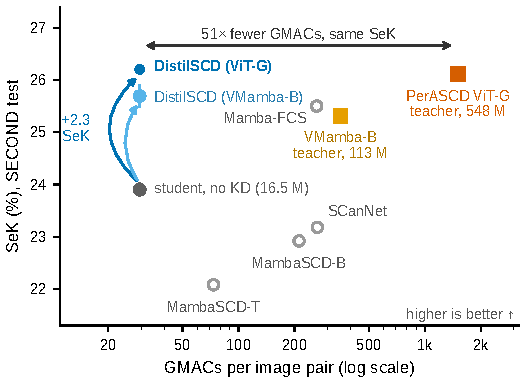
\includegraphics[width=\columnwidth]{fig1_sek_vs_gmacs}
\caption{Accuracy versus inference cost on the SECOND test set (official split). Distillation
moves the \StudentParams\,M-parameter student from \SecBaseSek\ to \SecFullSek\ SeK with the
ViT-G teacher and to \SecVmbSek\ with the VMamba-B teacher, at unchanged cost. Students: mean
over seeds of the best test epoch (field convention; last-epoch values in
Table~\ref{tab:second}); teachers: published checkpoints re-evaluated by us. Our models and the
teachers are counted with the same counter (PyTorch aten), which gives the \RatioGmacs$\times$
ratio; published models (open circles) are placed at their published complexity, an
fvcore-style MAC count, so the two groups of counts are not strictly comparable. SCanNet: as
retrained on the official split by~\cite{shen2026foundation}.}
\label{fig:pitch}
\end{figure}

This paper makes the following contributions.
\begin{enumerate}
\item \emph{DistilSCD, an output-only distillation recipe for SCD.} A frozen foundation-model
teacher is run once, offline, under the eight D4 views that the student's augmentation
produces; its change logits and class distributions supervise the student through a soft
binary cross-entropy and a temperature-scaled KL term. The student's architecture and
inference cost are unchanged, and training takes the same time as without distillation
(Section~\ref{sec:method}).
\item \emph{A controlled evaluation on SECOND.} With distillation hyper-parameters selected on an
internal validation split and five seeds on the test set, a \StudentParams\,M-parameter student
gains \SecFullGain\ SeK and is equivalent to the \TeacherParams\,M-parameter teacher within
$\pm\TostMargin$ SeK at \RatioGmacs$\times$ fewer MACs. A second, smaller and ImageNet-pretrained
teacher yields a smaller gain, and its student exceeds it (Section~\ref{sec:second}).
\item \emph{A train--test overlap analysis and a location-disjoint protocol for Landsat-SCD.} We verify at
the pixel level that the dataset holds \LkDistinct\ distinct images recombined into 2\,385
pairs, and release a four-fold cross-validation in which test tiles are never seen in
training (Section~\ref{sec:landsat-data}).
\item \emph{Evidence on where the gain comes from, and its limits.} Under the location-disjoint
protocol the distilled student improves on its undistilled counterpart on every fold and seed and
exceeds the single-run fold teachers. On SECOND, ground-truth change targets of the same form give
no gain, and our feature-distillation term adds nothing on top of output distillation. We discuss
which alternative explanations these controls leave open
(Sections~\ref{sec:landsat}--\ref{sec:discussion}).
\end{enumerate}
Code, splits, the overlap-verification script and the run logs are released (see Data and Code
Availability).

% =====================================================================================
\section{Related Work}
\label{sec:related}

\subsection{Semantic Change Detection}
HRSCD~\cite{daudt2019multitask} framed SCD as joint land-cover mapping and change detection.
Yang \emph{et al.}~\cite{yang2022asymmetric} introduced the SECOND dataset, an asymmetric
siamese network and the separated kappa (SeK) metric used throughout this paper. Bi-SRNet
\cite{ding2022bi} and SCanNet~\cite{ding2024joint} added bi-temporal semantic reasoning and
spatio-temporal Transformer modelling, and ChangeMask~\cite{zheng2022changemask} decoupled
semantic and change branches. State-space models entered the field with ChangeMamba
\cite{chen2024changemamba}, built on Mamba~\cite{gu2023mamba} and VMamba
\cite{liu2024vmamba}, and were followed by Mamba-FCS~\cite{wijenayake2026mamba} and GSTM-SCD
\cite{liu2025gstm}. The strongest recent results use foundation-model encoders: PerASCD
\cite{shen2026foundation}, DBTANet~\cite{li2026dual} with a SAM branch, and SemDINO
\cite{tong2026semdino}. Lightweight change detection has mostly been pursued by architecture
design for binary change~\cite{codegoni2023tinycd,li2023lightweight,cui2022shuffle}; Corley
\emph{et al.}~\cite{corley2024change} caution that well-trained simple baselines remain
competitive. We propose no new architecture: our contribution is a training signal and an
evaluation protocol.

\subsection{Foundation Models for Remote Sensing and Change Detection}
Remote-sensing foundation models are pre-trained by masked image modelling or contrastive
objectives on large archives~\cite{cong2022satmae,reed2023scale,sun2023ringmo,
wang2023advancing,manas2021seasonal,bastani2023satlaspretrain,fuller2023croma,
hong2024spectralgpt,jakubik2023foundation,guo2024skysense,xiong2024neural,wang2024mtp,
shen2026contrastive}. For change detection they are usually kept inside the deployed network,
either fine-tuned~\cite{shen2026foundation,ding2024adapting,li2024new,chen2024time,
dong2024changeclip,li2026dual} or used zero-shot~\cite{zheng2024segment}. Benchmarking studies
report that such comparisons are sensitive to evaluation details~\cite{marsocci2024pangaea,
corley2024revisiting}; we encountered the same sensitivity when reproducing a published
teacher (Section~\ref{sec:teachers}). Here the foundation model is used only at training
time.

\subsection{Knowledge Distillation}
Output distillation~\cite{hinton2015distilling} and its feature-based variants
\cite{romero2014fitnets,zagoruyko2016paying,park2019relational,tian2020contrastive,
zhao2022decoupled} are surveyed in~\cite{gou2021knowledge}. Two lines of results bear on our
setting. First, the \emph{capacity gap}: larger teachers do not always make better teachers
for small students~\cite{cho2019efficacy,mirzadeh2020improved,huang2022knowledge}, although
Beyer \emph{et al.}~\cite{beyer2022knowledge} show that consistent teaching (teacher and
student see the same view) and long schedules close much of the gap. Our D4 cache makes teaching
geometrically consistent, akin to stored per-crop soft labels~\cite{shen2022fast,yun2021re};
photometric jitter is applied to the student only, so teaching is not fully consistent in their
sense. Second, students can outperform their teachers
\cite{furlanello2018born,xie2020self,yuan2020revisiting}, and students that generalise well
may match their teachers poorly~\cite{stanton2021knowledge}; Yuan \emph{et al.}
\cite{yuan2020revisiting} interpret part of KD as a learned label smoothing
\cite{szegedy2016rethinking,muller2019label}. For dense prediction, structured and
channel-wise distillation transfer spatial structure for segmentation
\cite{liu2019structured,liu2023structured,shu2021channel,yang2022cross}. Closest to our
recipe in general vision, Vemulapalli \emph{et al.}~\cite{vemulapalli2024knowledge} fine-tune
a vision foundation model on the target task before distilling it into a small task model.

\subsection{Distillation in Remote Sensing and Change Detection}
KD in remote sensing is surveyed in~\cite{himeur2025applications}. For change detection, CDKD
\cite{wang2024knowledge} distils a large teacher's output probabilities, with contrastive and
normalised terms, into a lightweight on-board binary detector, and several works align
features between large and small binary change detectors~\cite{wang2025bi,yang2026intrascale,
wu2024lightweight}. Burden-free distillation (BFD)~\cite{wang2025burden} is the closest in
aim: it transfers features of generic vision foundation models into binary change detectors
and removes the foundation model at inference. Other teacher--student work targets accuracy
or robustness rather than compression: multi-teacher distillation~\cite{liu2026jl1},
self-distillation~\cite{liu2025novel,qu2026semantic,pang2024hicd}, weak supervision
\cite{lu2024weakly}, and GUIDE~\cite{huang2026guide}, a teacher--student framework for SCD
under cross-temporal domain shift. Relative to this work, we study \emph{semantic} change
detection on SECOND and Landsat-SCD, distil only the \emph{outputs} of a task-fine-tuned
remote-sensing foundation model, and test where the gain comes from with ground-truth target
controls, two teachers and location-disjoint folds.

\subsection{Evaluation Leakage and Spatial Validation}
Random splits of spatially or temporally dependent samples inflate accuracy; blocked or
spatial cross-validation is the remedy~\cite{roberts2017crossvalidation,ploton2020spatial,
meyer2021predicting,meyer2022machine}. In remote sensing, spatial dependence between training
and test samples is a documented pitfall of accuracy assessment~\cite{lyons2018comparison,
karasiak2022spatial,kattenborn2022spatially,olofsson2014good}. Kapoor and Narayanan
\cite{kapoor2023leakage} classify non-independence between training and test samples as
leakage unless the scientific claim concerns a distribution with the same dependence
structure. That qualification frames our treatment of Landsat-SCD: its random split is a valid
protocol for change recognition over one already-seen area, and we change the question to
generalisation to unseen locations. Reusing a test set for model selection biases reported
accuracy~\cite{dwork2015reusable,recht2019imagenet}, which motivates reporting a
selection-free number next to the field's convention, and seed variance motivates paired
multi-seed comparisons~\cite{bouthillier2021accounting}.

% =====================================================================================
\section{Method}
\label{sec:method}

Fig.~\ref{fig:method} summarises DistilSCD.

\begin{figure*}[t]
\centering
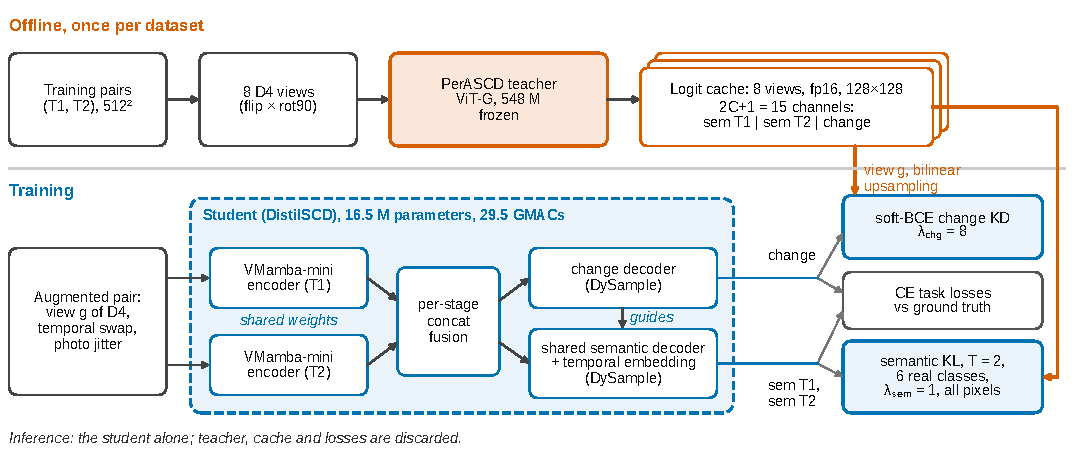
\includegraphics[width=\textwidth]{fig2_method}
\caption{DistilSCD. Offline and once per dataset, the frozen teacher is run on the eight $D_4$ views of
every training pair; its $2C+1$ output channels (class logits of both dates, class 0 = no change,
and a change logit) are stored at $128\times128$ in half precision. During training, the cache
entry of the view drawn by the student's augmentation is upsampled bilinearly and supervises the
student through a soft-target BCE on the change logit ($\lambda_{\mathrm{chg}}=8$) and a
temperature-scaled KL on the class distributions renormalised over the real classes
($T_{\mathrm{s}}=2$, $\lambda_{\mathrm{sem}}=1$, all pixels), in addition to the task losses. Only
the student is used at inference. Blocks inherited from the student's earlier design with no
measurable effect are omitted (supplementary material).}
\label{fig:method}
\end{figure*}

\subsection{Task and Notation}
An input is a co-registered image pair $(x^{1},x^{2})$ of size $H\times W$. The labels are a
binary change map $y^{\mathrm{c}}\in\{0,1\}^{H\times W}$ and two semantic maps
$y^{1},y^{2}\in\{0,\dots,C-1\}^{H\times W}$, where class $0$ denotes ``no change'' (no
semantic label) and classes $1,\dots,C-1$ are land-cover classes, defined only on changed
pixels. SECOND has $C=7$ (six land-cover classes); Landsat-SCD has $C=5$ (four classes).

\subsection{Student}
\label{sec:student}
The student is a compact siamese network developed by the first author before this study and
kept frozen in design and recipe throughout. A shared VMamba encoder~\cite{liu2024vmamba} with
depths $(2,2,5,2)$, widths $(96,192,384,768)$ and the MLP sub-blocks disabled (``mini'',
\num{13.84}\,M parameters) processes each date and is initialised from ImageNet VMamba-T
weights. Features of the two dates are fused per stage by concatenation and a $1\times1$
projection; a binary decoder predicts change logits $b\in\mathbb{R}^{2\times H\times W}$, and
a semantic decoder shared between the dates, conditioned on a learned temporal embedding and
on the change maps of the binary decoder, predicts class logits $s^{1},s^{2}\in\mathbb{R}^{C
\times H\times W}$. Both decoders use depth-wise refinement and DySample
upsampling~\cite{liu2023upsample}. The model has \StudentParams\,M parameters and
\StudentGmacs\ GMACs per $512\times512$ pair (\StudentGmacsFvcore\ with fvcore).
Two blocks inherited from the student's earlier design (a frequency branch and a change-guided
attention) have no established effect on SECOND; they are kept unchanged and documented in the
supplementary material, together with the design experiments, which selected epochs on the
SECOND test set as is customary on this dataset.

The task loss is
\begin{equation}
\begin{split}
\mathcal{L}_{\mathrm{task}} ={}& \mathrm{CE}(b,y^{\mathrm{c}})
 + \lambda_{\mathrm{sc}}\,\mathcal{L}_{\mathrm{sc}}\\
 &+ \tfrac12\big[\mathrm{CE}_{\neq0}(s^{1},y^{1})+\mathrm{CE}_{\neq0}(s^{2},y^{2})\big],
\end{split}
\label{eq:task}
\end{equation}
where $\mathrm{CE}_{\neq0}$ ignores class-0 pixels and $\mathcal{L}_{\mathrm{sc}}$
($\lambda_{\mathrm{sc}}=0.1$) is the bi-temporal feature-consistency loss of
Bi-SRNet~\cite{ding2022bi}.

\subsection{Teachers}
\label{sec:teacher-arch}
The main teacher is the published SECOND checkpoint of PerASCD~\cite{shen2026foundation}: a
PerA ViT-G/16 encoder (width 1024, 40 blocks)~\cite{shen2026contrastive}, a ViT-Adapter
\cite{chen2023vision} and a cascade gated decoder, \TeacherParams\,M parameters in total. It
outputs, at $1/4$ resolution, class logits $z^{1},z^{2}\in\mathbb{R}^{C\times h\times w}$ for
each date and a change logit $z^{\mathrm{c}}\in\mathbb{R}^{h\times w}$, which it upsamples
bilinearly to full resolution. The second teacher, released by the same authors, replaces the
encoder with VMamba-B (\num{113.01}\,M parameters). Both are frozen.

\subsection{Offline, View-Consistent Logit Cache}
\label{sec:cache}
The student is trained with horizontal and vertical flips and $90^\circ$ rotations, so each
training sample is seen under one of the eight elements $g$ of the dihedral group $D_4$. The
teacher is not equivariant to these transforms: on SECOND, its change decision for
$T(g\cdot x)$ and $g\cdot T(x)$ differs on 2.2--2.5\,\% of all pixels (about 20\,\% of the pixels are changed), and its class
decision on 2.7--3.0\,\% of the changed pixels. We
therefore run the teacher once on every training pair under all eight views and store the
$2C+1$ output channels at their native $1/4$ resolution in half precision (about 12\,GB for
the 2\,968 SECOND pairs, computed in 26 GPU-minutes). During training, the cache entry of the
drawn view $g$ supervises the augmented sample, so teacher and student always see the same
geometry; when the two dates are swapped (temporal-swap augmentation), the two semantic
blocks of the target are swapped and the symmetric change logit is kept. Photometric jitter is
applied to the student's input only, which adds a radiometric invariance constraint and makes
teaching photometrically inconsistent. We did not ablate the eight-view cache against a single
view. The
cached logits are upsampled bilinearly to the student's resolution, exactly as the teacher's
own last operation.

\subsection{Distillation Losses}
\label{sec:losses}
\emph{Change distillation.} With the student's change logit $d=b_{1}-b_{0}$ and temperature
$T_{\mathrm{c}}$,
\begin{equation}
\mathcal{L}_{\mathrm{chg}} = T_{\mathrm{c}}^{2}\;\mathrm{BCE}\!\left(\sigma(d/T_{\mathrm{c}}),
\;\sigma(z^{\mathrm{c}}/T_{\mathrm{c}})\right),
\end{equation}
averaged over all pixels (the change map is supervised everywhere). We use
$T_{\mathrm{c}}=1$.

\emph{Semantic distillation.} Class 0 is never a target of the teacher's cross-entropy, so its
logit carries no supervised meaning. We renormalise both distributions over the real classes
$1,\dots,C-1$:
\begin{equation}
\mathcal{L}_{\mathrm{sem}} = \frac{T_{\mathrm{s}}^{2}}{2}\sum_{t\in\{1,2\}}
\frac{1}{|\mathcal{M}|}\sum_{u\in\mathcal{M}}
\mathrm{KL}\!\left(q^{t}_{u}\,\Vert\,p^{t}_{u}\right),
\end{equation}
with $q^{t}=\mathrm{softmax}(z^{t}_{1:C-1}/T_{\mathrm{s}})$ and
$p^{t}=\mathrm{softmax}(s^{t}_{1:C-1}/T_{\mathrm{s}})$. The mask $\mathcal{M}$ is either the
whole image or the pixels predicted changed by the ground truth or the teacher; on SECOND,
about 80\,\% of pixels have no semantic label, so the first option asks the student to follow
the teacher's semantics where neither model was supervised.

\emph{Objective.} $\mathcal{L}=\mathcal{L}_{\mathrm{task}}+\lambda_{\mathrm{chg}}
\mathcal{L}_{\mathrm{chg}}+\lambda_{\mathrm{sem}}\mathcal{L}_{\mathrm{sem}}$. The retained
configuration, selected as described in Section~\ref{sec:screening}, is
$\lambda_{\mathrm{chg}}=8$, $\lambda_{\mathrm{sem}}=1$, $T_{\mathrm{s}}=2$ and
$\mathcal{M}=$ all pixels. We also screened one feature-distillation term (cosine similarity after channel-wise
normalisation between $1\times1$-projected student features and the teacher's encoder features at
two or three scales) on top of output distillation; it requires running the teacher online.

\subsection{Training Recipe}
\label{sec:recipe}
All students, with and without distillation, use the same recipe: full $512\times512$ tiles,
micro-batch 2 with 4 accumulation steps (effective batch 8), AdamW (learning rate
$10^{-4}$, weight decay $0.01$) with a 1\,500-iteration linear warm-up and a constant rate
afterwards, bfloat16 autocast, an exponential moving average of the weights (decay 0.9998)
used for evaluation, flips, $90^\circ$ rotations, photometric jitter (strength 0.2) and
temporal swap (probability 0.5). The budget is 120 epochs on SECOND (44\,520 optimiser steps)
and 100 epochs on Landsat-SCD (Section~\ref{sec:landsat-protocol}). The constant rate comes from the student's design campaign; with it, a shorter run is exactly a
prefix of a longer one; the seven no-distillation SECOND
seeds were trained for 200 epochs and are read at epoch 120. Distillation adds no measurable student training time, since the teacher never runs during
student training; the teacher's cost is paid once, when the cache is computed (and, on
Landsat-SCD, when the fold teachers are trained).

% =====================================================================================
\section{Datasets and Evaluation Protocol}
\label{sec:protocol}
Table~\ref{tab:datasets} summarises the datasets, splits and model-selection rules.

% generated by paper/scripts/make_tables_tex.py from paper/tables/*.csv -- do not edit
\begin{table*}[!t]
\centering
\footnotesize
\caption{Datasets and evaluation protocols (number of image pairs).}
\label{tab:datasets}
\setlength{\tabcolsep}{4pt}
\begin{tabular}{llrrrl}
\toprule
Dataset & Protocol & Train & Val & Test & Selection / remark \\
\midrule
SECOND & official split & 2\,968 & -- & 1\,694 & max test SeK over epochs and final epoch \\
SECOND & internal validation (screening) & 2\,671 & 297 & -- & max validation SeK; test never used \\
Landsat-SCD & released random pair split & 1\,431 & 477 & 477 & test pairs with both images in train: 477/477 \\
Landsat-SCD & location-disjoint fold 0 (exploratory) & 1\,603 & 202 & 580 & test tiles 00, 02, 20; val tile 21 \\
Landsat-SCD & location-disjoint fold 1 & 1\,590 & 202 & 593 & test tiles 01, 21, 30; val tile 12 \\
Landsat-SCD & location-disjoint fold 2 & 1\,590 & 189 & 606 & test tiles 10, 12, 22; val tile 02 \\
Landsat-SCD & location-disjoint fold 3 & 1\,577 & 202 & 606 & test tiles 11, 31, 32; val tile 10 \\
\bottomrule
\end{tabular}
\par\smallskip\parbox{\textwidth}{\scriptsize Landsat-SCD holds 333 distinct images at 12 locations, recombined into pairs. Location-disjoint folds: each location is a test location in exactly one fold; test at the epoch of best validation SeK of the fold. SECOND has no official validation split.}
\end{table*}


\subsection{SECOND}
SECOND~\cite{yang2022asymmetric} contains 4\,662 pairs of $512\times512$ aerial images with six
land-cover classes, split officially into 2\,968 training and 1\,694 test pairs; there is no
official validation split. Several papers evaluate on a split of the public training set
instead of the official test set~\cite{ding2022bi,ding2024joint}; we use the official split
throughout and compare only with results obtained on it. A pixel-hash check found no exact
duplicate image between the SECOND training and test sets.

\subsection{Landsat-SCD and Its Structure}
\label{sec:landsat-data}
Landsat-SCD~\cite{yuan2022transformer} covers a single area of Tumushuke, China, at 30\,m
resolution, with 28 acquisition dates between 1990 and 2020 and four land-cover classes
(farmland, desert, building, water). We use the $512\times512$ version distributed with
PerASCD, which removes the offline-augmented copies of the original release and keeps 2\,385
pairs split at random into 1\,431/477/477 for training, validation and test.

Pair names encode two years and a tile index $k$ taking only 12 values. A name-independent,
pixel-level verification (Table~\ref{tab:leakage}) shows that the 2\,385 pairs are built from
\LkDistinct\ distinct images, i.e. 12 tiles observed at about 28 dates, and that each
(tile, year) group contains exactly one image. As a consequence, all \LkTest\ test pairs, and
all \LkVal\ validation pairs, have both of their images in the training set, with identical
class labels on the \LkPixels\,M annotated pixels they share. A learning-free lookup that
copies, for each test pixel, the classes annotated for the same tile and year in the training
set reaches \LkOracleSek\ SeK on the test set (Fscd \LkOracleFscd, mIoU \LkOracleMiou), higher
than the published Landsat-SCD results we are aware of, which were obtained on random pair splits
(e.g. \PerascdLandsat\ for PerASCD~\cite{shen2026foundation}). Each image appears in about 14
pairs; when 60\,\% of the pairs are drawn at random for training, the probability that a test image
appears in none of the training pairs is about $0.4^{13}<10^{-5}$, so any random pair split has
this property, whatever its seed. We verified it on the released split only.

This is not an error of a particular paper. The original authors split pairs at random by
design~\cite[p.~11]{yuan2022transformer}, for a dataset built as a long time series of one
area, and name the extension to several regions as future work~\cite[p.~19]{yuan2022transformer}.
The random split measures change recognition on an area already seen at other dates; it does
not measure generalisation to a new area. Our student illustrates the difference
(Fig.~\ref{fig:leakage}b): on the random split its test SeK keeps rising, from
\RndTwoFifty\ at 250 epochs to \RndSixHundred\ at 600 epochs, with the validation curve still
climbing by \RndLastSlope\ points per 10 epochs at the end, whereas on unseen tiles it
plateaus below 30 SeK within 100 epochs.

% generated by paper/scripts/make_tables_tex.py from paper/tables/*.csv -- do not edit
\begin{table}[!t]
\centering
\footnotesize
\caption{Train--test image overlap in the released Landsat-SCD random pair split (LandsatSCD512).}
\label{tab:leakage}
\setlength{\tabcolsep}{4pt}
\begin{tabular}{@{}p{0.76\columnwidth}r@{}}
\toprule
Check & Value \\
\midrule
Image slots (2 images $\times$ 2385 pairs) & 4\,770 \\
Distinct images by pixel hash & 333 \\
Tile indices k (locations) & 12 \\
Val pairs with both images present in train & 477\,/\,477 \\
Test pairs with both images present in train & 477\,/\,477 \\
(k, year) groups with a single distinct image & 333\,/\,333 \\
Annotated pixels compared across duplicates & 198\,829\,642 \\
Class agreement on those pixels (\%) & 100.0 \\
Lookup oracle SeK on test (no learning) & 77.87 \\
Lookup oracle Fscd on test & 95.04 \\
Lookup oracle mIoU on test & 94.25 \\
Test changed pixels whose two classes are known from train (\%) & 90.8 \\
SECOND exact train/test duplicates (5936 train, 3388 test images) & 0 \\
\bottomrule
\end{tabular}
\par\smallskip\parbox{\columnwidth}{\scriptsize From scripts/verify\_landsat\_leakage.py (pixel hashes of every image slot). The lookup oracle predicts each test pair by looking up the training labels of the same two images, without learning. Last row: same check on SECOND.}
\end{table}


\begin{figure*}[t]
\centering
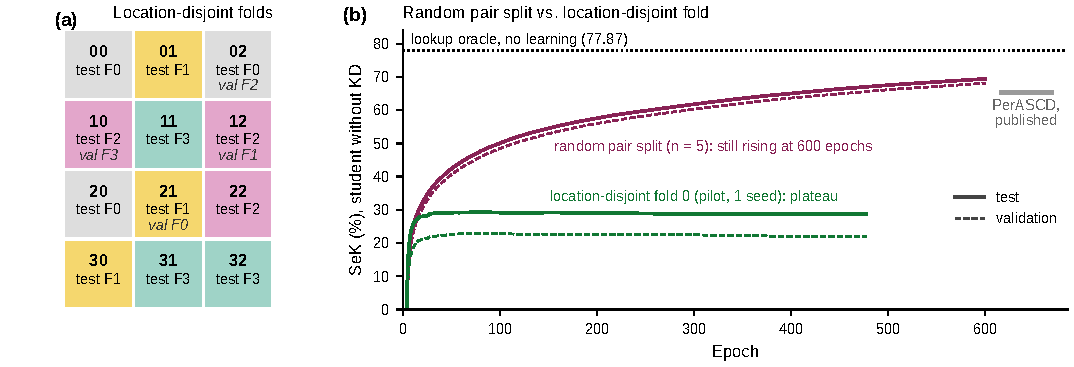
\includegraphics[width=\textwidth]{fig5_landsat_protocol}
\caption{Landsat-SCD: train--test image overlap of the released random pair split, and location-disjoint
protocol. (a) The
12 tile indices $k$ drawn as a $4\times3$ grid (row = first digit, column = second digit; the
layout is inferred from the indices, not from georeferencing), coloured by the fold in which the
tile is a test tile; ``val F$i$'' marks the validation tile of fold $i$. Fold 0 is exploratory.
(b) Test (solid) and validation (dashed) SeK per epoch of the same undistilled student on the
released random split (mean of five seeds; \RndSixHundred\ at epoch 600, still rising) and on
location-disjoint fold 0 (one pilot seed, stopped at epoch 477). Dotted line: learning-free lookup
oracle (\LkOracleSek). Grey tick: PerASCD as published (\PerascdLandsat). The
two sets of numbers answer different questions and are not comparable.}
\label{fig:leakage}
\end{figure*}

\subsection{Location-Disjoint Cross-Validation on Landsat-SCD}
\label{sec:landsat-protocol}
We group pairs by tile and build four folds of three test tiles each, chosen by exhaustive
search over the 15\,400 partitions of the 12 tiles into four groups of three to balance the
transition types and the change ratio (test change ratio 0.184--0.191, overall 0.188). In each
fold, one of the nine remaining tiles serves as validation and eight as training; the training
code refuses to start if a tile appears in two subsets. Test sets hold 580 to 606 pairs. The
student's epoch budget was fixed once, on fold 0 and on validation only, as the first
50-epoch window in which the validation SeK slope fell below 0.05 points per 10 epochs
(epochs 50--99), giving 100 epochs for every arm and fold. The folds, the verification script
and the budget rule are released.

\subsection{Metrics, Model Selection and Statistics}
\label{sec:stats}
We report SeK~\cite{yang2022asymmetric}, the SCD F-score Fscd and the mIoU of the
change/no-change map, computed with one implementation that reproduces the published teacher
scores to within 0.004 points. Values are in percentage points.

\emph{Model selection.} On SECOND, which has no validation split, the field reports the best
test SeK over epochs~\cite{chen2024changemamba,shen2026foundation}. We report this number and,
next to it, the SeK at the last epoch, which involves no selection. On Landsat-SCD we report
the test SeK at the epoch of best validation SeK of the fold.

\emph{Statistics.} Each arm is trained with several seeds; a seed fixes initialisation, data
order and augmentation draws, so arms with the same seed share their first mini-batch exactly.
On SECOND we report Welch tests and 95\,\% confidence intervals for differences of means, paired
tests across seeds, and one-sample tests against the single-seed teacher. On Landsat-SCD, the
variation between folds (standard deviation \LFoldSd\ SeK between fold means of the
undistilled student) dwarfs the variation between seeds, so all comparisons are paired by fold
and seed, and the unit of inference is the fold: we report a $t$ interval over the fold means. As a
consistency check, not a test, we also count the fold--seed pairs with a positive difference
(seeds within a fold are not independent). To compare the distilled student with the single-run
teacher on SECOND we use an equivalence test (two one-sided tests, margin $\pm\TostMargin$ SeK),
which treats the teacher's score as fixed. GPU training is not bit-reproducible; replays of the
same configuration differ by up to 0.5 SeK on Landsat-SCD, which adds variance to each paired
difference.

\subsection{Screening Specified in Advance}
\label{sec:screening}
All distillation hyper-parameters were chosen on SECOND before any distillation run was evaluated
on the test set. The 2\,968 training pairs were split into 2\,671 for training and 297 for
validation (a fixed, hashed split). With two seeds per arm and 120 epochs, three waves fixed in
turn the change weight $\lambda_{\mathrm{chg}}$, the semantic term ($T_{\mathrm{s}}\in\{2,4\}$, two
masks) and the feature term (two sets of scales, two weights). Before each wave, the decision rule
(``best mean validation SeK; an increment counts if it exceeds 0.36 points'') was written in the
project's lab journal, which is versioned with the code; it is not a public registration. The
0.36-point threshold was derived for five test seeds and serves here as a ranking threshold, not
as a test. The $\lambda_{\mathrm{chg}}$ grid started at $\{0.5,1,2\}$ and was extended to $\{4,8\}$,
then to 16, because the best value lay at the edge of the grid. Two controls, run at
$\lambda_{\mathrm{chg}}=2$, replaced the teacher's change target by the ground truth, either binary
or average-pooled to the teacher's resolution and upsampled like it. The SECOND teacher was trained
by its authors on all 2\,968 training pairs, including our 297 validation pairs, which can favour
distillation over the controls on validation. The retained configuration was then retrained on all
2\,968 pairs with five seeds and evaluated on the test set with the field's protocol
(Section~\ref{sec:stats}).

\subsection{Teachers: Reproduction and Retraining}
\label{sec:teachers}
Re-evaluated with our code, the published PerASCD checkpoint gives \TeacherVitgSekExact\ SeK
on the SECOND test set (published: 26.11). The published VMamba-B checkpoint gives 23.73 with
the PerA normalisation used by the released evaluation code, and exactly its stored score,
\TeacherVmbSekExact, with ImageNet normalisation, which we therefore use. Both checkpoints were
selected by their authors on the test set and are single runs; the training log of the ViT-G
checkpoint reads 26.13 at its best epoch and 25.85 at its last epoch. No Landsat-SCD teacher trained
on unseen tiles exists, and the published one has seen our test images; we therefore retrained
one PerASCD ViT-G teacher per fold with the authors' recipe (50 epochs, SGD), selected on the
fold's validation tile. Activation checkpointing of the 40 ViT blocks, which leaves gradients
unchanged, fits training on a 40\,GB A100. Before caching each fold teacher, a gate specified in advance required its validation SeK to exceed the mean validation SeK of the three undistilled
students of that fold.

% =====================================================================================
\section{Results on SECOND}
\label{sec:second}

\subsection{Screening on the Validation Split}
Table~\ref{tab:screening} and Fig.~\ref{fig:screening} summarise the screening. Change
distillation alone raises the validation SeK with its weight up to $\lambda_{\mathrm{chg}}=8$
(\ScrLEight\ against \ScrWit\ without distillation; the differences between 2, 4 and 8 are within
two-seed noise) and plateaus beyond (\IncLSixteen\ at $\lambda_{\mathrm{chg}}=16$). The two ground-truth controls at
$\lambda_{\mathrm{chg}}=2$ give \ScrCtlGtDelta\ and \ScrCtlGtsDelta\ points, against
\ScrLTwoDelta\ for the teacher's targets at the same weight. For the change term, the gain is
therefore not explained by adding a change loss of that weight or by softened boundaries; the
controls were run only at $\lambda_{\mathrm{chg}}=2$, with two seeds, on validation.
Adding semantic distillation at $T_{\mathrm{s}}=2$ brings a further \IncSemTwoAll\ (all pixels)
or \IncSemTwoChg\ (changed pixels) points; $T_{\mathrm{s}}=4$ is weaker (\IncSemFourAll,
\IncSemFourChg). The two masks are equivalent within noise; the rule retained all pixels. Our feature-distillation term on top of
output distillation adds \IncFeatA, \IncFeatB\ and
\IncFeatC\ points for the three variants, below the 0.36-point threshold, while multiplying the training time by
2.3--2.4 and the GPU memory by four; it was not retained.

% generated by paper/scripts/make_tables_tex.py from paper/tables/*.csv -- do not edit
\begin{table*}[!t]
\centering
\footnotesize
\caption{Screening on the SECOND internal validation split.}
\label{tab:screening}
\setlength{\tabcolsep}{3pt}
\begin{tabular}{lcllcccrr}
\toprule
Arm & $\lambda_{\mathrm{chg}}$ & Semantic KL & Feature KD & SeK max & SeK final & $\Delta$ max vs no KD ($p$) & h/run & GB \\
\midrule
no KD & 0 & -- & -- & 23.61\,$\pm$\,0.30 & 23.25\,$\pm$\,0.26 & -- & 4.8 & 4.2 \\
\midrule
control: binary GT target & 2 & -- & -- & 23.65\,$\pm$\,0.07 & 22.78\,$\pm$\,0.14 & +0.04 (0.89) & 4.7 & 4.2 \\
control: smoothed GT target & 2 & -- & -- & 23.59\,$\pm$\,0.01 & 23.06\,$\pm$\,0.69 & $-$0.02 (0.94) & 4.7 & 4.2 \\
\midrule
change KD & 0.5 & -- & -- & 24.20\,$\pm$\,0.54 & 24.01\,$\pm$\,0.27 & +0.59 (0.04) & 4.8 & 4.2 \\
change KD & 1 & -- & -- & 24.86\,$\pm$\,0.46 & 24.66\,$\pm$\,0.17 & +1.25 ($<$0.001) & 4.9 & 4.2 \\
change KD & 2 & -- & -- & 25.44\,$\pm$\,0.21 & 25.31\,$\pm$\,0.03 & +1.83 ($<$0.001) & 4.7 & 4.2 \\
change KD & 4 & -- & -- & 25.53\,$\pm$\,0.34 & 25.49\,$\pm$\,0.30 & +1.92 ($<$0.001) & 4.7 & 4.2 \\
change KD & 8 & -- & -- & 25.95\,$\pm$\,0.40 & 25.79\,$\pm$\,0.44 & +2.33 ($<$0.001) & 4.7 & 4.2 \\
change KD & 16 & -- & -- & 25.88\,$\pm$\,0.01 & 25.82\,$\pm$\,0.03 & +2.26 ($<$0.001) & 4.7 & 4.2 \\
\midrule
\textbf{DistilSCD} (output KD) & 8 & T = 2, all & -- & 26.74\,$\pm$\,0.06 & 26.66\,$\pm$\,0.13 & +3.13 ($<$0.001) & 4.7 & 4.2 \\
output KD & 8 & T = 2, changed & -- & 26.70\,$\pm$\,0.12 & 26.69\,$\pm$\,0.13 & +3.09 ($<$0.001) & 4.7 & 4.2 \\
output KD & 8 & T = 4, all & -- & 26.40\,$\pm$\,0.18 & 26.28\,$\pm$\,0.02 & +2.79 ($<$0.001) & 4.7 & 4.2 \\
output KD & 8 & T = 4, changed & -- & 26.46\,$\pm$\,0.31 & 26.45\,$\pm$\,0.32 & +2.85 ($<$0.001) & 4.7 & 4.2 \\
\midrule
+ feature KD & 8 & T = 2, all & 1/8, 1/16; 1 & 26.76\,$\pm$\,0.15 & 26.67\,$\pm$\,0.25 & +3.15 ($<$0.001) & 11.2 & 17.4 \\
+ feature KD & 8 & T = 2, all & 1/8, 1/16; 4 & 26.29\,$\pm$\,0.14 & 26.29\,$\pm$\,0.14 & +2.68 ($<$0.001) & 10.8 & 17.4 \\
+ feature KD & 8 & T = 2, all & 1/8, 1/16, 1/32; 1 & 26.86\,$\pm$\,0.20 & 26.82\,$\pm$\,0.13 & +3.25 ($<$0.001) & 10.7 & 17.4 \\
\bottomrule
\end{tabular}
\par\smallskip\parbox{\textwidth}{\scriptsize 16 arms $\times$ 2 seeds (1, 2) = 32 runs, 120 epochs, trained on 2\,671 SECOND training pairs and evaluated on the 297-pair internal validation split (the test set was not used). Mean $\pm$ standard deviation. $\Delta$: difference of the mean max SeK to the no-KD arm, with the $p$-value of a pooled-variance $t$-test. Controls replace the teacher's change target by the binary or smoothed ground truth, same loss and weight. Feature KD: encoder stages (fraction of the input resolution) and weight $\lambda_{\mathrm{feat}}$, on top of the retained output KD.}
\end{table*}


\begin{figure*}[t]
\centering
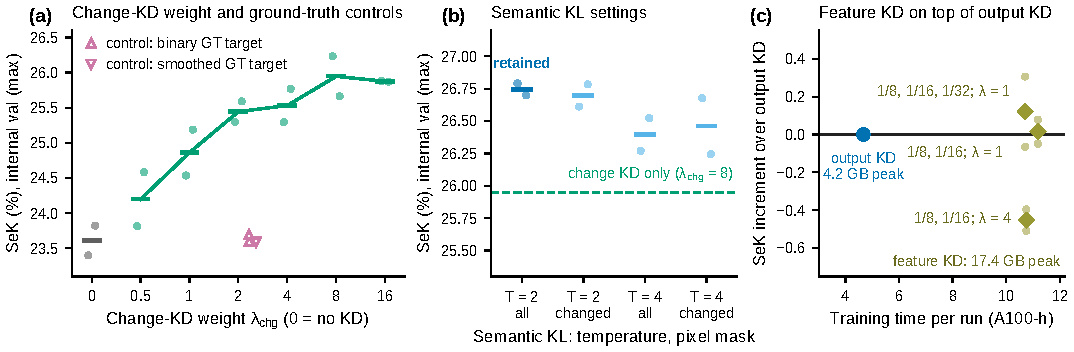
\includegraphics[width=\textwidth]{fig4_screening}
\caption{Screening on the SECOND internal validation split (2\,671/297 pairs;
the test set was not used); points are seeds (two per arm), ticks are means, $y$ is the best
validation SeK over 120 epochs. (a) Weight of the change term; the two controls at
$\lambda_{\mathrm{chg}}=2$ replace the teacher's target by the binary or the smoothed ground truth.
(b) Semantic KL on top of change distillation ($\lambda_{\mathrm{chg}}=8$, dashed line): temperature
and pixel mask. (c) Feature distillation on top of the retained output distillation: increment
paired by seed versus training time per run.}
\label{fig:screening}
\end{figure*}

\subsection{Test Confirmation}
\label{sec:second-test}
Table~\ref{tab:second} and Fig.~\ref{fig:second} report the test results. Without
distillation, the student reaches \SecBaseSek\,$\pm$\,\SecBaseSekSd\ SeK (best epoch,
$n=\SecBaseN$) and \SecBaseSekFinal\ at the last epoch. Change distillation alone gives
\SecChgSek\,$\pm$\,\SecChgSekSd\ (+\SecChgGain\ [\SecChgGainLo, \SecChgGainHi]). The full recipe
gives \SecFullSek\,$\pm$\,\SecFullSekSd\ (+\SecFullGain\ [\SecFullGainLo, \SecFullGainHi],
Welch $p\SecFullGainP$), with Fscd \SecFullFscd\ and mIoU \SecFullMiou. The semantic term
contributes +\SemInc\ [\SemIncLo, \SemIncHi] points paired by seed ($p\SemIncP$, \SemIncPos\
seeds positive). The selection-free last-epoch number tells the same story: \SecFullSekFinal\
against \SecBaseSekFinal\ (+\SecFullGainFinal\ [\SecFullGainFinalLo, \SecFullGainFinalHi]).
The
distilled student's best and final SeK differ by at most \SecFullMaxFinalGap\ points (best epochs
\SecFullBestEpMin--\SecFullBestEpMax), whereas the undistilled student peaks between epochs
\SecBaseBestEpMin\ and \SecBaseBestEpMax\ and then declines under the constant learning rate
(Fig.~\ref{fig:second}b). Distillation thus raises the peak and removes the late decline; a
decaying learning-rate schedule might remove part of that decline without distillation, which we
did not test, so we base the gain on the best-epoch number.

Against the teacher (\TeacherVitgSek), the distilled student differs by \SecFullVsT\
[\SecFullVsTLo, \SecFullVsTHi] SeK; its 90\,\% interval [\TostLo, \TostHi] lies within
$\pm\TostMargin$ SeK, so the two are equivalent at that margin (two one-sided tests, $p\TostP$),
treating the single-run teacher as fixed. Against the teacher's selection-free last-epoch value
(25.85), the student's last-epoch SeK (\SecFullSekFinal) is higher.
Its Fscd is slightly below the teacher's (66.41) and its mIoU slightly above (74.33).
Because the distilled runs were still improving at epoch 120, we resumed them to 200 epochs,
a decision taken after seeing the test curves and reported as a post-hoc extension: they reach
\SecFullTwoHundredSek\,$\pm$\,\SecFullTwoHundredSekSd\ (\SecFullTwoHundredVsT\
[\SecFullTwoHundredVsTLo, \SecFullTwoHundredVsTHi] above the teacher, $p\SecFullTwoHundredVsTP$)
and plateau after about 150 epochs, while the undistilled student's best epoch is unchanged and
its final SeK drops to \SecBaseSekFinalTwoHundred.

% generated by paper/scripts/make_tables_tex.py from paper/tables/*.csv -- do not edit
\begin{table*}[!t]
\centering
\footnotesize
\caption{Results on the SECOND test set.}
\label{tab:second}
\setlength{\tabcolsep}{3.2pt}
\begin{tabular}{lrccccccc}
\toprule
Model & $n$ & SeK max & SeK final & Fscd & mIoU & Gain [95\,\% CI] & $-$ teacher [95\,\% CI] & $p$ \\
\midrule
Student, no KD & 7 & 23.90\,$\pm$\,0.15 & 23.65\,$\pm$\,0.22 & 64.42\,$\pm$\,0.16 & 73.23\,$\pm$\,0.08 & -- & -- & -- \\
Change KD only (ViT-G) & 5 & 25.59\,$\pm$\,0.13 & 25.57\,$\pm$\,0.13 & 65.62\,$\pm$\,0.14 & 74.37\,$\pm$\,0.06 & +1.69 [1.51, 1.88] & $-$0.52 [$-$0.68, $-$0.35] & $<$0.001 \\
\textbf{DistilSCD (ViT-G)} & 5 & 26.20\,$\pm$\,0.11 & 26.20\,$\pm$\,0.11 & 66.29\,$\pm$\,0.11 & 74.57\,$\pm$\,0.05 & +2.30 [2.13, 2.47] & +0.09 [$-$0.04, 0.23] & 0.13 \\
DistilSCD (VMamba-B) & 5 & 25.69\,$\pm$\,0.17 & 25.69\,$\pm$\,0.18 & 65.73\,$\pm$\,0.14 & 74.38\,$\pm$\,0.09 & +1.79 [1.57, 2.01] & +0.38 [0.16, 0.59] & 0.009 \\
\midrule
Teacher ViT-G (548\,M) & 1 & 26.11 & -- & 66.41 & 74.33 & -- & -- & -- \\
Teacher VMamba-B (113\,M) & 1 & 25.31 & -- & 65.61 & 74.01 & -- & -- & -- \\
\bottomrule
\end{tabular}
\par\smallskip\parbox{\textwidth}{\scriptsize Mean $\pm$ standard deviation over seeds, 120 epochs. SeK max: maximum test SeK over epochs (field convention, as in ChangeMamba and PerASCD); Fscd and mIoU at that epoch. SeK final: last epoch, no selection. Gain: Welch difference of SeK max to the no-KD student. $-$ teacher: one-sample difference of SeK max to the teacher of the arm (ViT-G for change KD), with its $p$-value. Final-epoch gains are given in the text. Teachers: published checkpoints re-evaluated under our protocol, single run. Post-hoc 200-epoch extension of DistilSCD (ViT-G): 26.32\,$\pm$\,0.11 (Supplement).}
\end{table*}


\begin{figure*}[t]
\centering
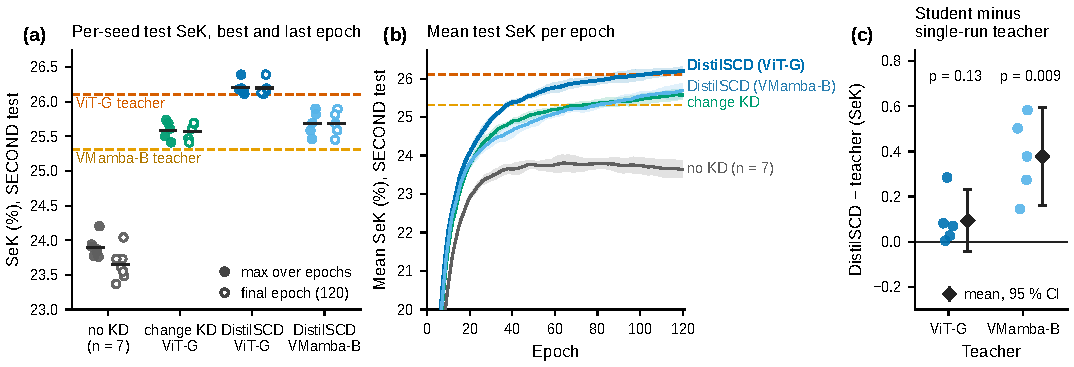
\includegraphics[width=\textwidth]{fig3_second_evidence}
\caption{SECOND test results. (a) Per-seed test SeK, best epoch (filled) and last epoch (open),
for the student without distillation ($n=\SecBaseN$), change-only distillation and DistilSCD
with each teacher ($n=5$); ticks are means; dashed lines are the single-run teachers. (b) Mean
test SeK per epoch (band: $\pm1$ s.d. across seeds); the undistilled curves are the first 120
epochs of 200-epoch constant-rate runs. (c) DistilSCD minus teacher per seed, with mean and
95\,\% interval: \SecFullVsT\ with ViT-G, \SecVmbVsT\ with VMamba-B; teachers are single runs.}
\label{fig:second}
\end{figure*}

\subsection{A Second, Smaller Teacher}
With the same recipe and no re-tuning, the VMamba-B teacher (\TeacherVmbSek\ SeK,
\num{113.01}\,M parameters, ImageNet-pretrained rather than a remote-sensing foundation
model) yields a student at \SecVmbSek\,$\pm$\,\SecVmbSekSd, which exceeds that single-run teacher by \SecVmbVsT\ [\SecVmbVsTLo, \SecVmbVsTHi] ($p\SecVmbVsTP$). The ViT-G teacher, more
accurate and $33\times$ the student's size, yields the better student:
+\TeacherDiff\ [\TeacherDiffLo, \TeacherDiffHi] SeK paired by seed ($p\TeacherDiffP$,
\TeacherDiffPos\ seeds). The two teachers differ at once in size, architecture, pre-training and accuracy, so this
comparison does not test the capacity-gap hypothesis~\cite{cho2019efficacy,mirzadeh2020improved};
it shows only that a much larger teacher did not yield a worse student here.

\subsection{Efficiency}
Table~\ref{tab:efficiency} compares the two models on the same A100 at $512\times512$ (median
of 50 runs after 10 warm-up runs). With the same operation counter on both models, the student
needs \RatioGmacs$\times$ fewer MACs (\StudentGmacs\ against \TeacherGmacs\ GMACs; the counter
omits the student's selective scan and the teacher's deformable attention, both small). The
latency advantage is smaller: \RatioLatFpThirtyTwo$\times$ in float32 and \RatioLatBf$\times$ in
bfloat16 at batch size 8, \RatioLatOneFpThirtyTwo$\times$ at batch size 1 in float32. The
teacher benefits from tensor cores in half precision, whereas the student is limited by memory
accesses; latency, which governs deployment, does not follow the MAC count. Peak memory at
batch size 8 is \StudentMem\ against \TeacherMem\,GB.

% generated by paper/scripts/make_tables_tex.py from paper/tables/*.csv -- do not edit
\begin{table}[!t]
\centering
\footnotesize
\caption{Efficiency of DistilSCD and its ViT-G teacher on one A100 GPU: (a) inference, (b) training cost per run (120 epochs).}
\label{tab:efficiency}
\textit{(a) Inference}\par\smallskip
\setlength{\tabcolsep}{4pt}
\begin{tabular}{lrrr}
\toprule
Quantity & DistilSCD & Teacher & Ratio \\
\midrule
Parameters (M) & 16.5 & 548.2 & 33.3$\times$ \\
GMACs / pair (aten counter) & 29.48 & 1509.74 & 51.2$\times$ \\
GMACs / pair (fvcore) & 31.42 & -- & -- \\
Latency b8 fp32 (ms) & 129.4 & 1613.4 & 12.5$\times$ \\
Latency b8 bf16 (ms) & 113.7 & 561.1 & 4.9$\times$ \\
Latency b8 fp16 (ms) & 112.6 & 487.1 & 4.3$\times$ \\
Latency b1 fp32 (ms) & 26.3 & 268.5 & 10.2$\times$ \\
Latency b1 bf16 (ms) & 30.2 & 125.6 & 4.2$\times$ \\
Peak memory b8 fp32 (GB) & 1.96 & 25.09 & 12.8$\times$ \\
Peak memory b8 bf16 (GB) & 1.82 & 26.09 & 14.3$\times$ \\
\bottomrule
\end{tabular}
\par\smallskip\parbox{\columnwidth}{\scriptsize Same job and GPU for both models; 512$\times$512 pairs; median latency; b8 / b1: batch of 8 / 1 pair(s). The teacher's fvcore count failed (JIT tracing of bicubic interpolation). Both counters ignore custom CUDA operators.}
\par\medskip
\textit{(b) Training}\par\smallskip
\setlength{\tabcolsep}{3pt}
\begin{tabular}{@{}llrrrr@{}}
\toprule
Prot. & Arm & Runs & h/run & s/epoch & GB \\
\midrule
confirm. & change KD & 5 & 6.38 & 149.3 & 4.23 \\
confirm. & DistilSCD (output KD) & 5 & 6.43 & 150.5 & 4.23 \\
screen. & no KD & 2 & 4.84 & 138.7 & 4.23 \\
screen. & DistilSCD (output KD) & 2 & 4.67 & 133.4 & 4.23 \\
screen. & + feat. KD 1/8, 1/16; 1 & 2 & 11.19 & 319.9 & 17.42 \\
screen. & + feat. KD 1/8--1/32; 1 & 2 & 10.71 & 316.3 & 17.43 \\
screen. & + feat. KD 1/8, 1/16; 4 & 2 & 10.76 & 317.4 & 17.42 \\
\bottomrule
\end{tabular}
\par\smallskip\parbox{\columnwidth}{\scriptsize Pairs used (confirm.: 2968 train, test set as validation; screen.: 2671 train, 297 val). GB: peak training memory. From the run timing logs. Output KD reads the offline logit cache and adds no measurable training time; feature KD runs the teacher online.}
\end{table}


\subsection{Comparison with Published Results}
Fig.~\ref{fig:pitch} and Table~\ref{tab:published} place the distilled student among published
SECOND results obtained on the official split. Published values are taken from the papers.
ChangeMamba and Mamba-FCS report fvcore counts labelled ``GFLOPs'', which count
multiply--accumulates, so we plot them as GMACs; conventions are not uniform across papers
(PerASCD reports 2853 ``GFLOPs'' for the model we measure at \TeacherGmacs\ GMACs), so cross-paper
costs are indicative only. The distilled student reaches the accuracy level of the foundation-model
teacher at the lowest compute in the table. Published accuracies are single numbers whose
selection rules are not always stated.



% generated by paper/scripts/make_tables_tex.py from paper/tables/*.csv -- do not edit
\begin{table*}[!t]
\centering
\footnotesize
\caption{Comparison with published results on the SECOND test set.}
\label{tab:published}
\setlength{\tabcolsep}{4pt}
\begin{tabular}{lrrlrrrl}
\toprule
Model & Params (M) & GMACs & Counter & SeK & Fscd & mIoU & Provenance \\
\midrule
PerASCD, ViT-G (teacher)~\cite{shen2026foundation} & 548.17 & 1509.74 & aten & 26.11 & 66.41 & 74.33 & re-evaluated \\
Mamba-FCS~\cite{wijenayake2026mamba} & 189.54 & 263.15 & paper & 25.50 & 65.78 & 74.07 & reported, checked \\
VMamba-B + CG-Decoder (teacher)~\cite{shen2026foundation} & 113.01 & 352.90 & aten & 25.31 & 65.61 & 74.01 & re-evaluated \\
MambaSCD-Tiny, released ckpt.$^{a}$ & 37.13 & 115.44 & fvcore$^{a}$ & 23.34 & -- & -- & measured \\
SCanNet~\cite{ding2024joint} (retrained by PerASCD)$^{b}$ & 27.90 & 264.95 & paper & 23.18 & 63.53 & 73.03 & reported, checked \\
MambaSCD-Base~\cite{chen2024changemamba} & 89.99 & 211.55 & paper & 22.92 & --$^{c}$ & 73.68 & reported, checked \\
MambaSCD-Tiny~\cite{chen2024changemamba} & 21.51 & 73.42 & paper & 22.08 & --$^{c}$ & 73.33 & reported, checked \\
\midrule
Student, no KD & 16.48 & 29.48 & aten & 23.90 & 64.42 & 73.23 & ours, 7 seeds \\
\textbf{DistilSCD} (ViT-G teacher) & 16.48 & 29.48 & aten & 26.20 & 66.29 & 74.57 & ours, 5 seeds \\
DistilSCD (VMamba-B teacher) & 16.48 & 29.48 & aten & 25.69 & 65.73 & 74.38 & ours, 5 seeds \\
\bottomrule
\end{tabular}
\par\smallskip\parbox{\textwidth}{\scriptsize Params in M; GMACs per image pair at 512$\times$512. aten: torch.utils.flop\_counter, the same counter for our models and the teachers (measured by us); it counts neither the deformable attention of the teacher nor the selective scan of the student (fvcore gives 31.42 GMACs for the student). paper: complexity reported by the original papers as `GFLOPs', which are fvcore-style MAC counts for ChangeMamba and Mamba-FCS (conventions differ across papers); a different counter from aten, so not strictly comparable. Accuracies of published models as reported in their papers, on the official SECOND split. $^{a}$Released checkpoint evaluated with our metric code; params and fvcore GMACs measured by us; the released code builds a larger configuration than the one reported in the paper (row MambaSCD-Tiny). $^{b}$SCanNet retrained on the official split by the PerASCD authors (their Table I; params and GFLOPs from ChangeMamba Table VIII); the SeK reported in the SCanNet paper uses a different, non-official evaluation split and is not used. $^{c}$ChangeMamba reports an `F1' column whose values are not comparable with the Fscd of the other rows; omitted. Provenance: reported, checked = from the cited paper, checked against it; re-evaluated = published checkpoint evaluated under our protocol (SeK, Fscd, mIoU as published, SeK reproduced); measured = released checkpoint run with our code. Sources: PerASCD (arXiv 2602.13780, Table I), Mamba-FCS (arXiv 2508.08232, Tables V--VI), ChangeMamba (arXiv 2404.03425, Tables VII--VIII).}
\end{table*}


% =====================================================================================
\section{Results on Location-Disjoint Landsat-SCD}
\label{sec:landsat}

Table~\ref{tab:landsat} and Fig.~\ref{fig:landsat} report the four folds.

\emph{Teachers.} The retrained fold teachers pass the gate on folds 1--3 and fail
it on fold 0, where the teacher's validation SeK (21.85) is below that of the undistilled
students (22.50). On the test tiles, the teachers lead the undistilled students by \FOneTMinusB,
\FTwoTMinusB\ and \FThreeTMinusB\ SeK on folds 1--3 and trail by \FZeroTMinusB\ on fold 0, a mean
lead of \LTeacherMinusBMean\ points, far below the 2.2-point lead on SECOND. Because the rule fixed before training the teachers
caches only teachers that pass the gate, folds 1--3 form the primary analysis. We also ran fold 0 with the gate explicitly lifted and
marked as exploratory, and report it as a secondary analysis.

\emph{Distillation.} Distillation improves the student on every fold and every seed. On the
three primary folds, the test SeK rises by \LPrimGain\ points (95\,\% interval over fold means
[\LPrimGainLo, \LPrimGainHi], $p\LPrimGainP$; \LPrimPos\ fold--seed pairs positive), with Fscd +\LPrimFscd\ and mIoU +\LPrimMiou. Over all four folds the gain is
\LSecGain\ [\LSecGainLo, \LSecGainHi] ($p\LSecGainP$, \LSecPos\ pairs positive). Per fold, the
gains are \FOneGain, \FTwoGain\ and \FThreeGain\ on folds 1--3 and \FZeroGain\ on the exploratory
fold 0, where the teacher was no better than the student. The spread across seeds is smaller with distillation on three of the four
folds.

\emph{Distilled student versus teacher.} The distilled student exceeds its fold teacher on all
four folds, by \LPrimKdMinusT\ points on average over folds 1--3 ($p\LPrimKdMinusTP$ with three
folds) and \LSecKdMinusT\ over all four ($p\LSecKdMinusTP$). Each fold teacher is a single run,
trained with a recipe that its authors tuned on the random split and selected on a single
validation tile, so these teachers may be under-tuned. The comparison does not depend on how the
teachers' epoch was selected: the distilled students exceed even the teachers' best test epoch on
every fold, by at least \LKdMinusTMaxMin\ points (supplementary Table~SIV).

\emph{Budget.} The 100-epoch budget was fixed on undistilled students; it does not handicap
distillation: the validation SeK of the distilled runs changes by at most \LKdSlopeMax\ points
per 10 epochs over epochs 70--99, and the last-epoch test gain (\LPrimGainFinal\ on folds 1--3)
equals the gain at the selected epoch.

% generated by paper/scripts/make_tables_tex.py from paper/tables/*.csv -- do not edit
\begin{table*}[!t]
\centering
\footnotesize
\caption{Landsat-SCD, location-disjoint folds: test SeK.}
\label{tab:landsat}
\setlength{\tabcolsep}{4pt}
\begin{tabular}{llccccccc}
\toprule
Fold & Test tiles & Gate & Teacher & Student, no KD & DistilSCD & Gain & KD $-$ teacher & Teacher $-$ student \\
\midrule
0$^{\dagger}$ & 00, 02, 20 & no & 28.61 & 28.75\,$\pm$\,0.37 & \textbf{31.21\,$\pm$\,0.09} & +2.46 & +2.60 & $-$0.14 \\
1 & 01, 21, 30 & yes & 26.02 & 25.57\,$\pm$\,0.08 & \textbf{28.05\,$\pm$\,0.15} & +2.48 & +2.03 & +0.45 \\
2 & 10, 12, 22 & yes & 22.48 & 21.48\,$\pm$\,0.32 & \textbf{23.32\,$\pm$\,0.08} & +1.84 & +0.84 & +1.00 \\
3 & 11, 31, 32 & yes & 20.18 & 18.42\,$\pm$\,0.60 & \textbf{21.70\,$\pm$\,0.17} & +3.28 & +1.52 & +1.75 \\
\midrule
\multicolumn{3}{l}{Folds 1--3 (primary)} & 22.89 & 21.82 & 24.36 & +2.53 [0.74, 4.32] & +1.46 & +1.07 \\
\multicolumn{3}{l}{Folds 0--3 (secondary)} & 24.32 & 23.56 & 26.07 & +2.51 [1.58, 3.45] & +1.75 & +0.77 \\
\bottomrule
\end{tabular}
\par\smallskip\parbox{\textwidth}{\scriptsize Test SeK at the epoch of best validation SeK of the fold. Students: mean $\pm$ standard deviation over 3 seeds; teacher: PerASCD ViT-G retrained by us with the authors' recipe, one run per fold. Gain: KD $-$ no KD, paired by seed; fold means for the summary rows, with a 95\,\% CI across folds. Positive seed pairs: 9/9 (folds 1--3), 12/12 (folds 0--3; a consistency count, seeds within a fold are not independent). $^{\dagger}$Fold 0 failed the teacher gate specified in advance and was run with the gate lifted (exploratory).}
\end{table*}


\begin{figure*}[t]
\centering
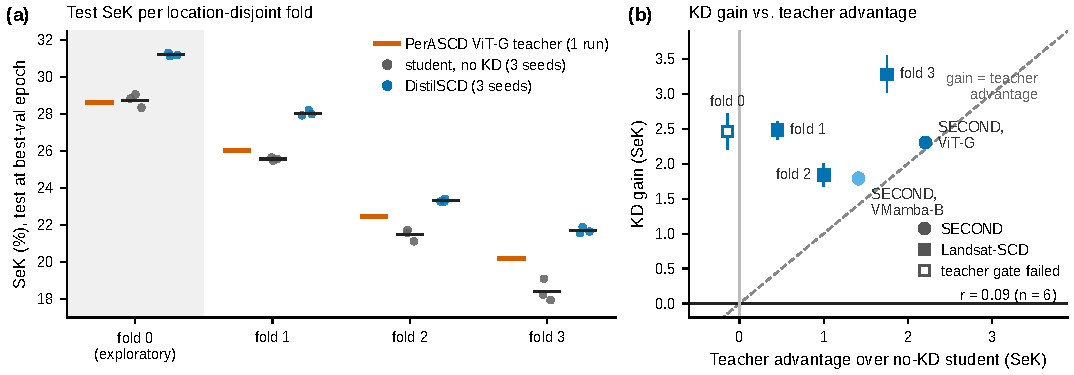
\includegraphics[width=\textwidth]{fig6_landsat_results}
\caption{Landsat-SCD, location-disjoint folds. (a) Test SeK at the epoch of best validation SeK:
fold teacher (one run), student without distillation and DistilSCD (three seeds each). Fold 0
(shaded) failed the teacher gate specified in advance and is exploratory. (b) Distillation gain versus
the teacher's advantage over the undistilled student, for six teacher--dataset configurations
(SECOND: best test epoch; Landsat-SCD: three seed pairs per fold); error bars: $\pm1$ s.e.; open
marker: fold 0; points above the dashed line are students that outscore their teacher.}
\label{fig:landsat}
\end{figure*}

% =====================================================================================
\section{Discussion}
\label{sec:discussion}

\subsection{Gain and Teacher Advantage}
One might expect distillation to help in proportion to how much better the teacher is than the
student. Within SECOND, the more accurate teacher (advantage \TeacherAdvVitg\ against
\TeacherAdvVmb\ SeK) does give the larger gain (+\TeacherDiff\ paired). Across our six
teacher--dataset configurations (Fig.~\ref{fig:landsat}b), however, the gain stays between 1.8 and
3.3 SeK while the teacher's advantage ranges from \FZeroTMinusB\ to 2.21, and on fold 0 a teacher
slightly worse than the student on the test tiles still yields +\FZeroGain\ points. Six
configurations from two datasets with different selection rules cannot establish that the gain is
independent of the teacher's advantage (correlation $r=\CorrR$, $n=\CorrN$); they do show that a
teacher need not outscore the student to help it. In hindsight, our gate (``the teacher must beat
the student on validation'') was conservative.

What, then, is transferred? Our evidence narrows the answer only partly. On SECOND, ground-truth
change targets with the same loss and weight, binary or with the teacher's softened boundaries,
give no gain on validation; these controls concern the change term only, at
$\lambda_{\mathrm{chg}}=2$ and with two seeds, and they smooth targets spatially, not across classes
as label smoothing does~\cite{szegedy2016rethinking,muller2019label}. The teacher's targets are not
a copy of the labels: on its own SECOND training set the teacher scores 33.24 SeK, and its semantic
predictions cover the 80\,\% of pixels that carry no label, where the semantic term acts. Our
results are consistent with reports that students benefit from teachers that are weak or no
better than themselves~\cite{furlanello2018born,yuan2020revisiting,stanton2021knowledge}, which
interpret part of distillation as learned regularisation. A self-distillation control (the
undistilled student as its own teacher, with the same cache and losses) and a class-level
label-smoothing control would separate knowledge transfer from regularisation; we did not run
them.

\subsection{Output Distillation and Our Feature Term}
Feature distillation is often reported to help dense prediction~\cite{liu2019structured,
shu2021channel}, and BFD~\cite{wang2025burden} distils foundation-model features into binary
change detectors. In our setting, once outputs are distilled, our feature term (cosine alignment of projected
student features with the ViT-G encoder features) adds nothing at the tested weights and scales,
and a larger weight hurts. We did not test feature distillation alone, other feature losses, or
the generic foundation-model features that BFD distils. Output distillation also has a practical advantage: it can be
computed offline, so the student's training cost is unchanged, whereas feature distillation
needs the teacher online (2.3$\times$ the training time and four times the memory here).

\subsection{What the Landsat-SCD Analysis Implies}
Landsat-SCD numbers computed on random pair splits, ours included, answer a recognition question
over a single, already-seen area. They remain meaningful for that question, but they should not be
read as generalisation to new areas: on the released split, a lookup table exceeds the published
models we compared. Under the location-disjoint protocol, scores drop to 18--31 SeK depending on the
fold, the fold-to-fold variation is large, and conclusions require paired designs. We release
the folds and the verification script so that future work can report both numbers.

\subsection{Limitations}
\label{sec:limitations}
Our evidence covers two datasets, one student architecture and two teachers on SECOND that differ
in several respects at once. Teachers are single runs: the published SECOND checkpoints, selected
by their authors on the test set, and one retrained teacher per Landsat-SCD fold, trained with a
recipe tuned by its authors on the random split. SECOND has no official validation split, so its
headline numbers follow the field's test-epoch convention; the selection-free last-epoch numbers
lead to the same conclusions. The student recipe was developed on SECOND, with test-epoch
selection, before this study and then frozen; it uses a constant learning rate, and we did not test
whether a decaying schedule would narrow the gap at the last epoch. The screening used two seeds
per arm; the ground-truth controls cover the change term only; self-distillation and
label-smoothing controls, other distillation losses and a single-view cache were not tested. Each
Landsat-SCD fold validates on a single tile, which makes model selection noisy, and the fold-0
analysis is exploratory. On Landsat-SCD, distillation first required training one
\TeacherParams\,M-parameter teacher per fold (\ComputeLandsatTeachers\ A100-hours in total). Finally, latency
gains (\RatioLatOneBf--\RatioLatFpThirtyTwo$\times$ on an A100) are much smaller than compute
gains (\RatioGmacs$\times$), because the student is limited by memory accesses.

% =====================================================================================
\section{Conclusion}
\label{sec:conclusion}
Distilling only the outputs of a \TeacherParams\,M-parameter remote-sensing foundation model into a
\StudentParams\,M-parameter student brings the student to the teacher's accuracy on SECOND
(equivalent within $\pm\TostMargin$ SeK) at \RatioGmacs$\times$ fewer MACs, without changing the
student or its inference cost. On Landsat-SCD, evaluating this required a location-disjoint
protocol, because the released random split places every test image in the training set; under
that protocol, distillation improves the student on every fold and seed and the distilled students
exceed their single-run fold teachers. The gain, 1.8 to 3.3 SeK across six configurations, appears
even where the teacher does not outscore the student. Future work should separate knowledge
transfer from regularisation with self-distillation and label-smoothing controls, test other
student families, and extend location-disjoint evaluation to other change detection benchmarks.

\section*{Data and Code Availability}
\label{sec:availability}
Code, training scripts, the SECOND internal validation split, the Landsat-SCD location-disjoint
folds, the overlap-verification script and the per-run logs are available at
\url{https://github.com/mathismagron/distilscd}. Student weights will be released once the licence
of the teacher weights has been clarified with their authors. The teacher checkpoints are those released by
the PerASCD authors; we do not redistribute them or the teachers we retrained from them.

\section*{Acknowledgment}
The authors thank the authors of PerASCD, ChangeMamba and Landsat-SCD for releasing their code,
data and checkpoints. Computations were enabled by the Digital Research Alliance of Canada.

\bibliographystyle{IEEEtran}
\bibliography{refs}

\end{document}
